% tags: arc edgeLabel label blockDiagram house background align
\PassOptionsToPackage{usenames,dvipsnames}{xcolor}
\documentclass[tikz, border=10pt]{standalone}

\usepackage{verbatim}
\usepackage{amsmath}

\tikzset{>=stealth}
\tikzstyle{every node}=[align=center]
\usetikzlibrary{spy,shadows,arrows,shapes,positioning,calc,backgrounds,fit,automata}

\newcommand{\Green}{OliveGreen!40}
\newcommand{\Yellow}{GreenYellow!70}
\newcommand{\Orange}{Orange!60}
\newcommand{\Brown}{Sepia!40}
\newcommand{\DarkGreen}{OliveGreen!60}
\newcommand{\DarkOrange}{Orange}
\newcommand{\DarkYellow}{GreenYellow!120}
\newcommand{\DarkBrown}{Sepia!60}
\begin{document}
\pgfdeclarelayer{bg}
\pgfdeclarelayer{fg}
\pgfsetlayers{bg,main,fg}
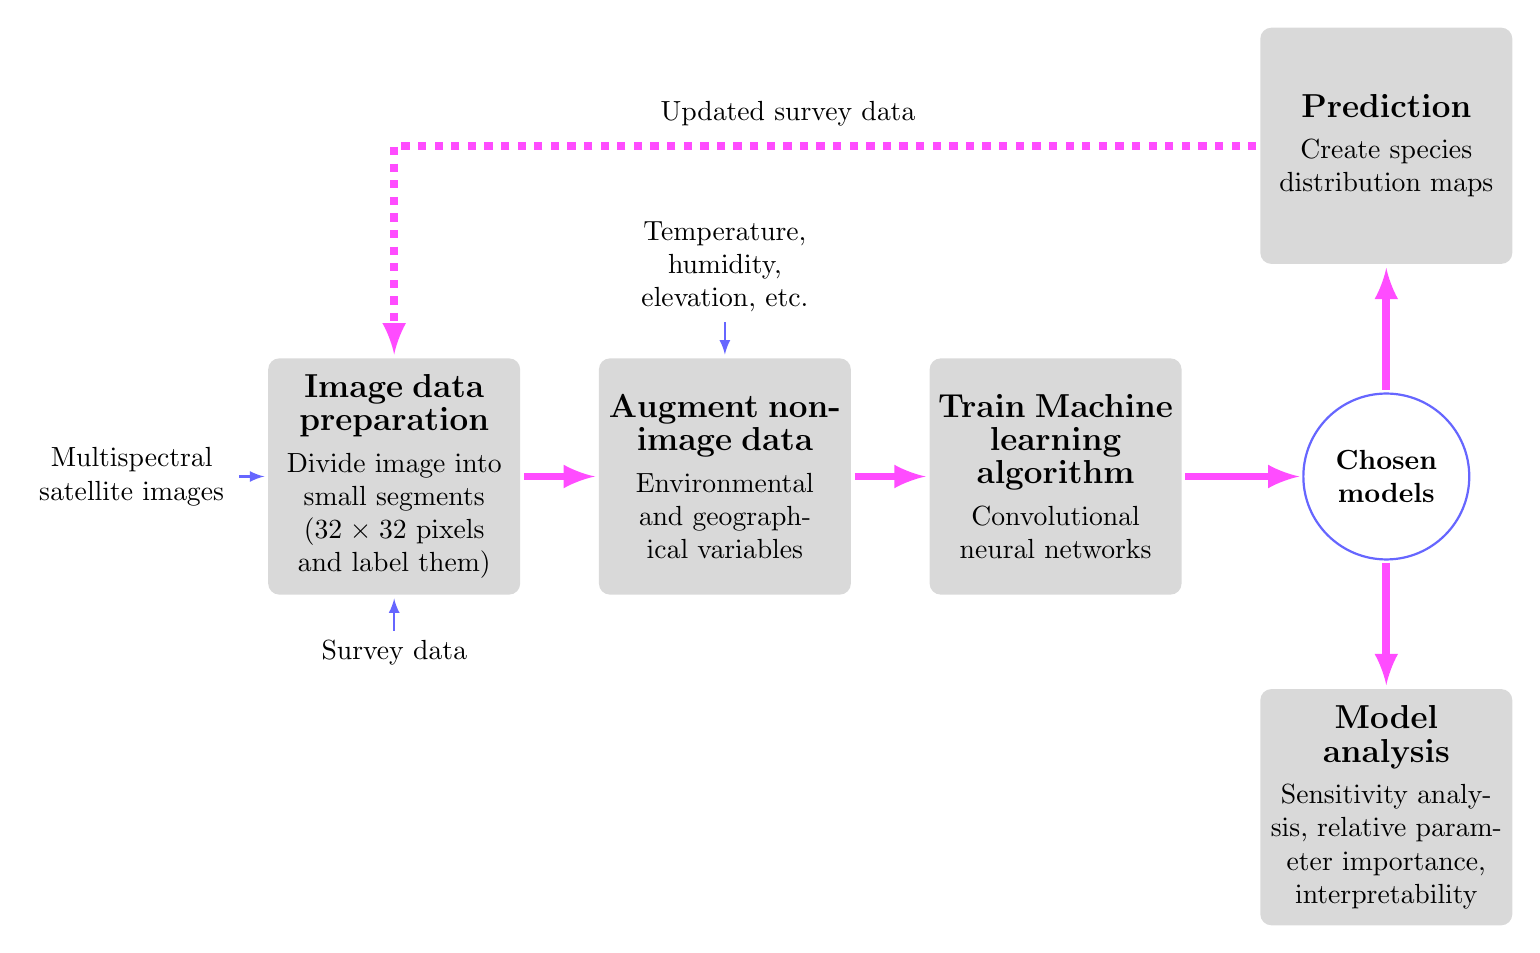
\begin{tikzpicture}
[
blk/.style={inner sep=.1cm,fill=black!15,rounded corners,text width=3cm,minimum height=3cm},
every node/.style={inner sep=0,align=center},
blkedge/.style={draw=Magenta!70,>=latex, shorten >=1pt, shorten <=1pt, line width=1mm},
datedge/.style={draw=Blue!60,>=latex, shorten >=1pt, shorten <=1pt}, 
node distance=4.2cm,thick
]

%% Data preparation
%% image prep
\node[blk,] (prep) {\textbf{\large Image data\\
preparation}\\\smallskip Divide image into small segments ($32\times 32$
pixels and label them)};
\draw[datedge,<-] (prep) -- +(-2,0) node[inner sep=2,text
width=2.5cm,anchor=east,align=center]{Multispectral satellite images};
\draw[datedge,<-] (prep) -- +(0,-2) node[inner sep=2,text
width=2.5cm,anchor=north,align=center]{Survey data};
%% Augment data
\node[blk,,right of=prep] (augment) {\textbf{\large Augment
non-image data} \\ \smallskip Environmental and geographical variables};
\draw[datedge,<-] (augment) -- +(0,2) node[inner sep=2,text
width=2.5cm,anchor=south,align=center]{Temperature, humidity, elevation,
etc.};
\draw[blkedge,->] (prep) -- (augment);
%% Train
\node[blk,,right of=augment] (train) {\textbf{\large Train
Machine learning algorithm} \\ \smallskip Convolutional neural networks};
\draw[blkedge,->] (augment) -- (train);
%% models
\node[circle,draw=Blue!60,right of=train,text width=2cm] (models)
{\textbf{Chosen \\models}};
\draw[blkedge,->] (train) -- (models);
%% predict
\node[blk,,above of=models] (predict) {\textbf{\large Prediction} \\
\smallskip Create species distribution maps};
\draw[blkedge,->] (models) -- (predict);
\draw[blkedge,->,dashed] (predict) -| (prep)
node[midway,above,shift={(5,.2)}] {Updated survey data};
%% analysis
\node[blk,,below of=models] (analysis) {\textbf{\large Model analysis} \\
\smallskip Sensitivity analysis, relative parameter importance,
interpretability};
\draw[blkedge,->] (models) -- (analysis);
\end{tikzpicture}
\end{document}
